\documentclass{article}%
\usepackage[T1]{fontenc}%
\usepackage[utf8]{inputenc}%
\usepackage{lmodern}%
\usepackage{textcomp}%
\usepackage{lastpage}%
\usepackage{geometry}%
\geometry{tmargin=2.5cm,rmargin=2.5cm,bmargin=2.5cm,lmargin=2.5cm}%
\usepackage{graphicx}%
%
\title{PrimAITE 3.0.0 Learning Benchmark}%
\author{PrimAITE Dev Team}%
\date{2024{-}06{-}01}%
%
\begin{document}%
\normalsize%
\maketitle%
\section{Introduction}%
\label{sec:Introduction}%
PrimAITE v3.0.0 was benchmarked automatically upon release. Learning rate metrics were captured to be referenced during system{-}level testing and user acceptance testing (UAT).%
\newline%
The benchmarking process consists of running 10 training session using the same config file. Each session trains an agent for 1000 episodes, with each episode consisting of 128 steps.%
\newline%
The mean reward per episode from each session is captured. This is then used to calculate a combined average reward per episode from the 10 individual sessions for smoothing. Finally, a 25{-}widow rolling average of the combined average reward per session is calculated for further smoothing.

%
\section{System Information}%
\label{sec:SystemInformation}%
\subsection{Python}%
\label{subsec:Python}%
\begin{tabular}{|l|l|}%
\hline%
\textbf{Version}&3.8.10 (tags/v3.8.10:3d8993a, May  3 2021, 11:48:03) {[}MSC v.1928 64 bit (AMD64){]}\\%
\hline%
\end{tabular}

%
\subsection{System}%
\label{subsec:System}%
\begin{tabular}{|l|l|}%
\hline%
\textbf{OS}&Windows\\%
\hline%
\textbf{OS Version}&10.0.19045\\%
\hline%
\textbf{Machine}&AMD64\\%
\hline%
\textbf{Processor}&Intel64 Family 6 Model 85 Stepping 4, GenuineIntel\\%
\hline%
\end{tabular}

%
\subsection{CPU}%
\label{subsec:CPU}%
\begin{tabular}{|l|l|}%
\hline%
\textbf{Physical Cores}&6\\%
\hline%
\textbf{Total Cores}&12\\%
\hline%
\textbf{Max Frequency}&3600.00Mhz\\%
\hline%
\end{tabular}

%
\subsection{Memory}%
\label{subsec:Memory}%
\begin{tabular}{|l|l|}%
\hline%
\textbf{Total}&63.52GB\\%
\hline%
\textbf{Swap Total}&9.50GB\\%
\hline%
\end{tabular}

%
\section{Stats}%
\label{sec:Stats}%
\subsection{Benchmark Results}%
\label{subsec:BenchmarkResults}%
\begin{tabular}{|l|l|}%
\hline%
\textbf{Total Sessions}&10\\%
\hline%
\textbf{Total Episodes}&10010\\%
\hline%
\textbf{Total Steps}&1280000\\%
\hline%
\textbf{Av Session Duration (s)}&1569.8775\\%
\hline%
\textbf{Av Step Duration (s)}&0.0012\\%
\hline%
\textbf{Av Duration per 100 Steps per 10 Nodes (s)}&0.1226\\%
\hline%
\end{tabular}

%
\section{Graphs}%
\label{sec:Graphs}%
\subsection{PrimAITE 3.0.0 Learning Benchmark Plot}%
\label{subsec:PrimAITE3.0.0LearningBenchmarkPlot}%


\begin{figure}[h!]%
\centering%
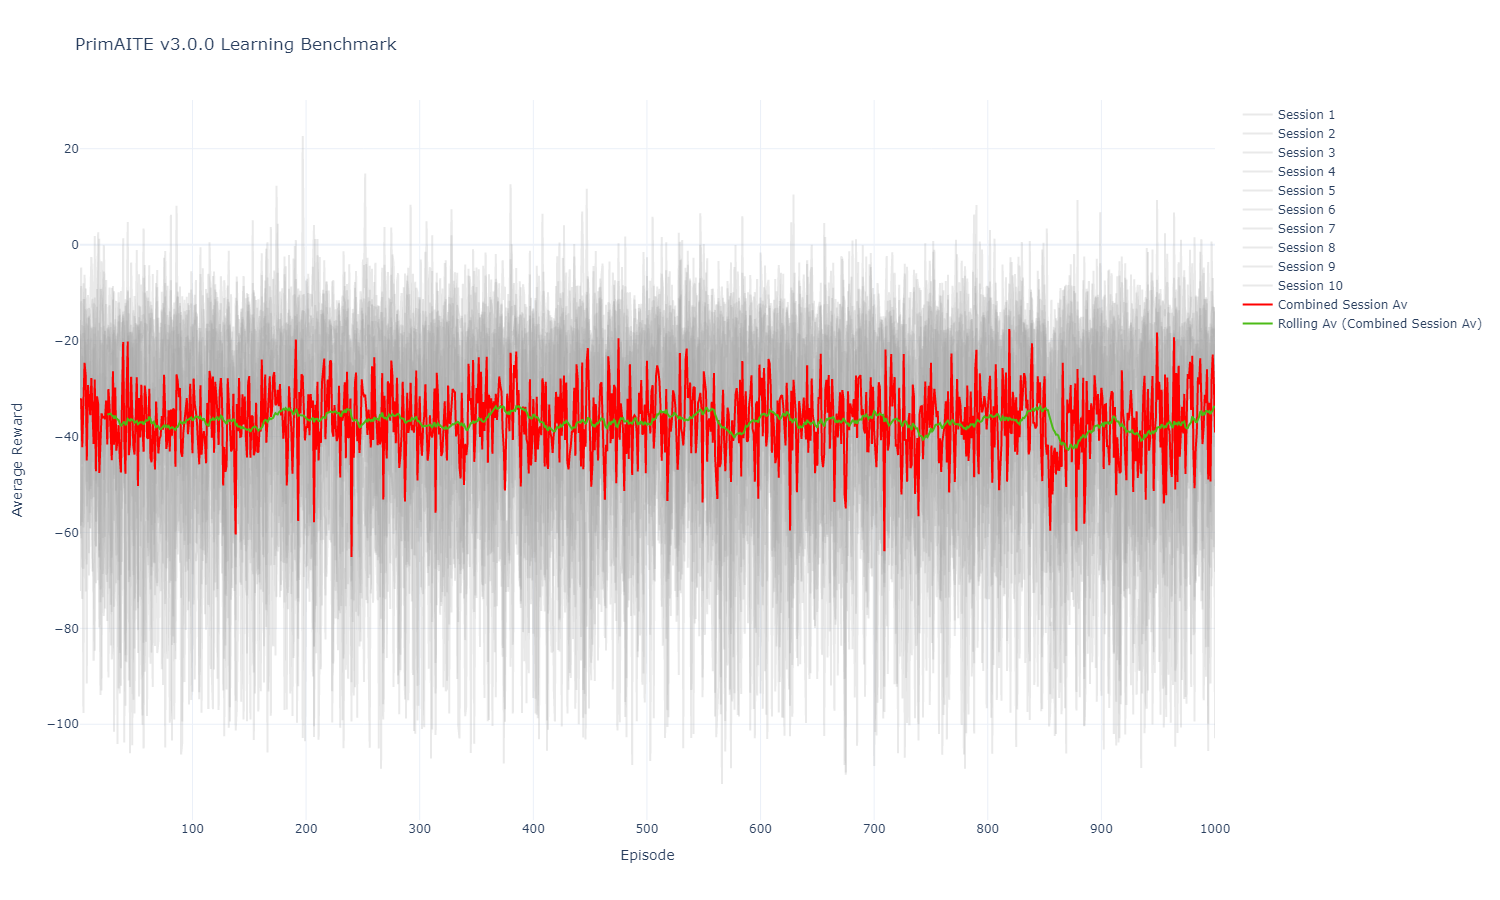
\includegraphics[width=0.8\textwidth]{D:/Projects/ARCD/PrimAITE/PrimAITE/benchmark/results/v3.0.0/PrimAITE v3.0.0 Learning Benchmark.png}%
\caption{PrimAITE 3.0.0 Learning Benchmark Plot}%
\end{figure}

%
\subsection{PrimAITE All Versions Learning Benchmark Plot}%
\label{subsec:PrimAITEAllVersionsLearningBenchmarkPlot}%


\begin{figure}[h!]%
\centering%
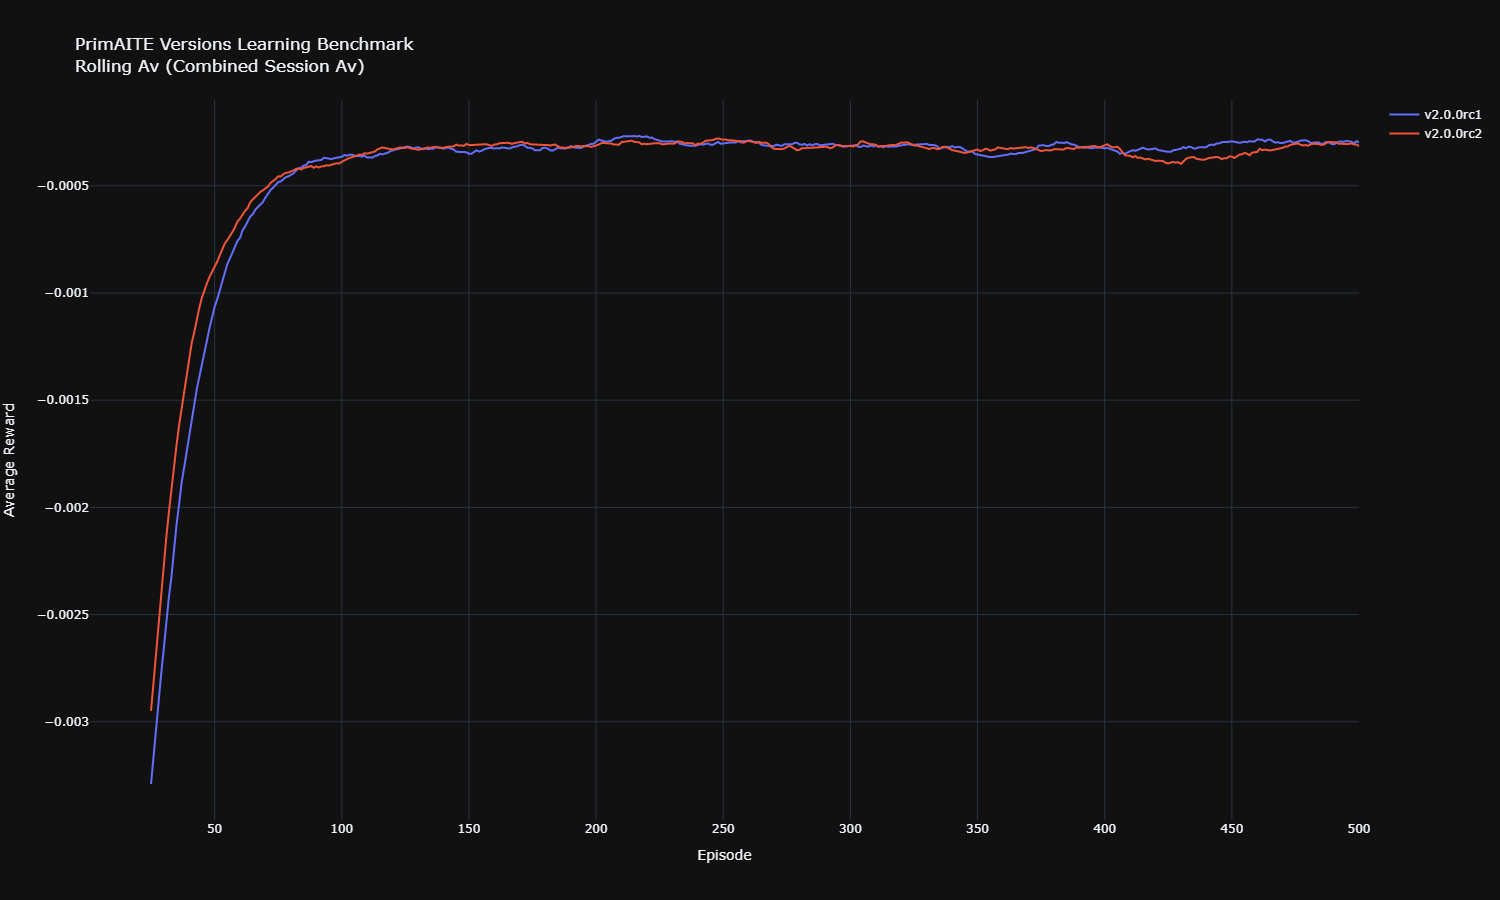
\includegraphics[width=0.8\textwidth]{D:/Projects/ARCD/PrimAITE/PrimAITE/benchmark/results/PrimAITE Versions Learning Benchmark.png}%
\caption{PrimAITE All Versions Learning Benchmark Plot}%
\end{figure}

%
\end{document}
